\documentclass{article}

\usepackage{amsmath,amssymb,amsthm}

\setlength{\oddsidemargin}{0.25 in}
\setlength{\evensidemargin}{-0.25 in}
\setlength{\topmargin}{-0.6 in}
\setlength{\textwidth}{6.5 in}
\setlength{\textheight}{8.5 in}
\setlength{\headsep}{0.75 in}
\setlength{\parindent}{0 in}
\setlength{\parskip}{0.1 in}

\newtheorem{theorem}{Theorem}
\newtheorem{corollary}{Corollary}
\newtheorem{proposition}{Proposition}
\newtheorem*{remark}{Remark}
\theoremstyle{definition}
\newtheorem{example}{Example}
\newtheorem{definition}{Definition}

\newcommand{\lecture}[4]{
   \pagestyle{myheadings}
   \thispagestyle{plain}
   \newpage
%   \setcounter{lecnum}{#1}
   \setcounter{page}{1}
   \noindent
   \begin{center}
   \framebox{
      \vbox{\vspace{2mm}
    \hbox to 6.58in { {\bf CSC~565: Graph Theory
                        \hfill North Carolina State University} }
    \hbox to 6.58in { {\bf Fall 2019
                        \hfill Computer Science} }
       \vspace{4mm}
       \hbox to 6.28in { {\Large \hfill Lecture #1: #2  \hfill} }
       \vspace{2mm}
       \hbox to 6.28in { {\it Lecturer: {\it Don Sheehy {\tt <drsheehy@ncsu.edu>}} \hfill Scribe: #4} }
      \vspace{2mm}}
   }
   \end{center}
   \markboth{Lecture #1: #2}{Lecture #1: #2}
   \vspace*{4mm}
}
\usepackage{graphics,tikz}
\def\geom{\text{geom}}
\def\sim{\text{sim}}
\def\R{\mathbb{R}}
\begin{document}


%FILL IN THE RIGHT INFO.
%\lecture{**LECTURE-NUMBER**}{**DATE**}{**LECTURER**}{**SCRIBE**}
\lecture{6}{Sep 11, 2019}{Don Sheehy}{John Watson, Vishnu Ramachandran, Zitong Li }

  % \title{Lecture 6}
  % \author{Scribed by: }
  % \maketitle
\section{Simplicial Map}
\begin{definition}
Let X and Y be simplicial complexes. A simplicial map $f: X \rightarrow Y$ is a pair of functions:
\centerline {$f_v: V_X \rightarrow V_Y$ and $f_S: S_X \rightarrow S_Y$}

where $f_S(\sigma) = \{ f_V(u): u \in \sigma \}$
\end{definition}

So, to get a simplicial map $f': simp(G) \rightarrow simp(H)$ from a graph morphism $f= (f_0, f_1)$ where $f_0: V_G \rightarrow V_H$ and $f_1: E_G \rightarrow E_H$, we simply define $f'_V = f_0$ and $f'_S(\sigma) = \{ f'_V(u): u \in \sigma \} = \{ f_0(u): u \in \sigma \}$
Note $f'_S$ maps vertices to vertices and edges to edges.

\begin{example}
In the following example, let G be the graph on the right and H on the left. The morphism can be defined as $$\begin{cases} f(A) = C \\ f(B) = D \end{cases}$$ The simplicial map can be defined as $\hat{f}$ = $(\hat{f_V}, \hat{f_S})$ where $$ \begin{cases} \hat{f_V}(A) = C \\ \hat{f_V}(B) = D \end{cases} $$ and $\hat{f_S}$ can be expressed as $$\begin{cases} \hat{f_S}(\emptyset) = \emptyset \\ \hat{f_S}(\{A\}) = \{C\} \\ \hat{f_S}(\{B\}) = \{D\} \\ \hat{f_S}(\{A,B\}) = \{C, D\} \end{cases} $$
\begin{figure}[!h]
\centering

\tikzset{every picture/.style={line width=0.75pt}} %set default line width to 0.75pt        

\begin{tikzpicture}[x=0.75pt,y=0.75pt,yscale=-1,xscale=1]
%uncomment if require: \path (0,127.19999694824219); %set diagram left start at 0, and has height of 127.19999694824219

%Straight Lines [id:da5385123876450288] 
\draw    (131,109) -- (206.3,26.2) ;
\draw [shift={(206.3,26.2)}, rotate = 312.28] [color={rgb, 255:red, 0; green, 0; blue, 0 }  ][fill={rgb, 255:red, 0; green, 0; blue, 0 }  ][line width=0.75]      (0, 0) circle [x radius= 3.35, y radius= 3.35]   ;
\draw [shift={(131,109)}, rotate = 312.28] [color={rgb, 255:red, 0; green, 0; blue, 0 }  ][fill={rgb, 255:red, 0; green, 0; blue, 0 }  ][line width=0.75]      (0, 0) circle [x radius= 3.35, y radius= 3.35]   ;
%Straight Lines [id:da49260056812167474] 
\draw    (492,21.2) -- (440.3,64.2) ;
\draw [shift={(440.3,64.2)}, rotate = 140.25] [color={rgb, 255:red, 0; green, 0; blue, 0 }  ][fill={rgb, 255:red, 0; green, 0; blue, 0 }  ][line width=0.75]      (0, 0) circle [x radius= 3.35, y radius= 3.35]   ;
\draw [shift={(492,21.2)}, rotate = 140.25] [color={rgb, 255:red, 0; green, 0; blue, 0 }  ][fill={rgb, 255:red, 0; green, 0; blue, 0 }  ][line width=0.75]      (0, 0) circle [x radius= 3.35, y radius= 3.35]   ;
%Straight Lines [id:da46232185123279357] 
\draw    (440.3,64.2) -- (494.3,116.2) ;
\draw [shift={(494.3,116.2)}, rotate = 43.92] [color={rgb, 255:red, 0; green, 0; blue, 0 }  ][fill={rgb, 255:red, 0; green, 0; blue, 0 }  ][line width=0.75]      (0, 0) circle [x radius= 3.35, y radius= 3.35]   ;


% Text Node
\draw (192,16) node  [align=left] {A};
% Text Node
\draw (118,112) node  [align=left] {B};
% Text Node
\draw (501,11) node  [align=left] {C};
% Text Node
\draw (423,63) node  [align=left] {D};
% Text Node
\draw (511,116) node  [align=left] {E};


\end{tikzpicture}

\end{figure}
\end{example}

\begin{definition}
A graph G is planer $\iff$ G has no $K_{3,3}$ or $K_5$ minor $\iff$ G has no $K_{3,3}$ or $K_5$ topological minor
\end{definition}

\begin{definition}
A is a \textit{minor} of B if there exists a surjective map $\sim(B) \to \sim(A)$ such that preimages are connected, i.e., $\forall v \in V_{a}$. \\
\\ Note :  What does connected mean for a simplicial complex?
\\ In this case $f^{-1}(v)$ is a set of vertices and edges. Every edge in $f^{-1}(v)$ has both ends in $f^{-1}(v)$ and so it can naturally be treated as a graph. 
\end{definition}
\begin{example}
Equivalently, we form a minor by contracting edges as can be seen in the diagram below.
\end{example}
\begin{figure}[!h]
\tikzset{every picture/.style={line width=0.75pt}} %set default line width to 0.75pt        

\begin{tikzpicture}[x=0.75pt,y=0.75pt,yscale=-1,xscale=1]
%uncomment if require: \path (0,300); %set diagram left start at 0, and has height of 300

%Shape: Circle [id:dp7874728646482212] 
\draw   (27.39,166.22) .. controls (27.39,159.25) and (33.04,153.61) .. (40,153.61) .. controls (46.96,153.61) and (52.61,159.25) .. (52.61,166.22) .. controls (52.61,173.18) and (46.96,178.82) .. (40,178.82) .. controls (33.04,178.82) and (27.39,173.18) .. (27.39,166.22) -- cycle ;
%Shape: Circle [id:dp6181673278518854] 
\draw  [color={rgb, 255:red, 208; green, 2; blue, 27 }  ,draw opacity=1 ] (94.78,85.61) .. controls (94.78,78.64) and (100.43,73) .. (107.39,73) .. controls (114.36,73) and (120,78.64) .. (120,85.61) .. controls (120,92.57) and (114.36,98.22) .. (107.39,98.22) .. controls (100.43,98.22) and (94.78,92.57) .. (94.78,85.61) -- cycle ;
%Shape: Circle [id:dp10240670692021347] 
\draw   (168.78,157.61) .. controls (168.78,150.64) and (174.43,145) .. (181.39,145) .. controls (188.36,145) and (194,150.64) .. (194,157.61) .. controls (194,164.57) and (188.36,170.22) .. (181.39,170.22) .. controls (174.43,170.22) and (168.78,164.57) .. (168.78,157.61) -- cycle ;
%Shape: Circle [id:dp4014047549827079] 
\draw  [color={rgb, 255:red, 208; green, 2; blue, 27 }  ,draw opacity=1 ] (86.78,140.61) .. controls (86.78,133.64) and (92.43,128) .. (99.39,128) .. controls (106.36,128) and (112,133.64) .. (112,140.61) .. controls (112,147.57) and (106.36,153.22) .. (99.39,153.22) .. controls (92.43,153.22) and (86.78,147.57) .. (86.78,140.61) -- cycle ;
%Shape: Circle [id:dp03668405154709242] 
\draw   (85.78,223.61) .. controls (85.78,216.64) and (91.43,211) .. (98.39,211) .. controls (105.36,211) and (111,216.64) .. (111,223.61) .. controls (111,230.57) and (105.36,236.22) .. (98.39,236.22) .. controls (91.43,236.22) and (85.78,230.57) .. (85.78,223.61) -- cycle ;
%Straight Lines [id:da9343930887466414] 
\draw    (40,153.61) -- (94.78,85.61) ;


%Straight Lines [id:da36808512921987246] 
\draw    (181.39,145) -- (120,85.61) ;


%Straight Lines [id:da19520669877000107] 
\draw    (111,223.61) -- (181.39,170.22) ;


%Straight Lines [id:da42310436229581805] 
\draw    (40,178.82) -- (85.78,223.61) ;


%Straight Lines [id:da547395758903153] 
\draw    (52.61,166.22) -- (86.78,140.61) ;


%Straight Lines [id:da20646247550939234] 
\draw    (168.78,157.61) -- (112,140.61) ;


%Straight Lines [id:da6712334623523222] 
\draw [color={rgb, 255:red, 208; green, 2; blue, 27 }  ,draw opacity=1 ]   (99.39,128) -- (107.39,98.22) ;


%Straight Lines [id:da6359698032382797] 
\draw    (214,144.22) -- (265,144.22) ;
\draw [shift={(267,144.22)}, rotate = 180] [color={rgb, 255:red, 0; green, 0; blue, 0 }  ][line width=0.75]    (10.93,-3.29) .. controls (6.95,-1.4) and (3.31,-0.3) .. (0,0) .. controls (3.31,0.3) and (6.95,1.4) .. (10.93,3.29)   ;

%Shape: Circle [id:dp711367673887124] 
\draw  [color={rgb, 255:red, 208; green, 2; blue, 27 }  ,draw opacity=1 ][fill={rgb, 255:red, 255; green, 255; blue, 255 }  ,fill opacity=1 ] (333.78,101.61) .. controls (333.78,94.64) and (339.43,89) .. (346.39,89) .. controls (353.36,89) and (359,94.64) .. (359,101.61) .. controls (359,108.57) and (353.36,114.22) .. (346.39,114.22) .. controls (339.43,114.22) and (333.78,108.57) .. (333.78,101.61) -- cycle ;
%Shape: Circle [id:dp7584671256479122] 
\draw   (349.78,188.61) .. controls (349.78,181.64) and (355.43,176) .. (362.39,176) .. controls (369.36,176) and (375,181.64) .. (375,188.61) .. controls (375,195.57) and (369.36,201.22) .. (362.39,201.22) .. controls (355.43,201.22) and (349.78,195.57) .. (349.78,188.61) -- cycle ;
%Shape: Circle [id:dp2348097164304196] 
\draw   (403.78,141.61) .. controls (403.78,134.64) and (409.43,129) .. (416.39,129) .. controls (423.36,129) and (429,134.64) .. (429,141.61) .. controls (429,148.57) and (423.36,154.22) .. (416.39,154.22) .. controls (409.43,154.22) and (403.78,148.57) .. (403.78,141.61) -- cycle ;
%Shape: Circle [id:dp8023815598854389] 
\draw   (281.78,149.61) .. controls (281.78,142.64) and (287.43,137) .. (294.39,137) .. controls (301.36,137) and (307,142.64) .. (307,149.61) .. controls (307,156.57) and (301.36,162.22) .. (294.39,162.22) .. controls (287.43,162.22) and (281.78,156.57) .. (281.78,149.61) -- cycle ;
%Straight Lines [id:da9077087154105346] 
\draw    (294.39,137) -- (333.78,101.61) ;


%Straight Lines [id:da010160860388972681] 
\draw    (416.39,129) -- (359,101.61) ;


%Straight Lines [id:da7873481965861147] 
\draw    (375,188.61) -- (416.39,154.22) ;


%Shape: Circle [id:dp7175206681298579] 
\draw   (559.78,96.61) .. controls (559.78,89.64) and (565.43,84) .. (572.39,84) .. controls (579.36,84) and (585,89.64) .. (585,96.61) .. controls (585,103.57) and (579.36,109.22) .. (572.39,109.22) .. controls (565.43,109.22) and (559.78,103.57) .. (559.78,96.61) -- cycle ;
%Shape: Circle [id:dp12565042665387371] 
\draw   (603.78,163.61) .. controls (603.78,156.64) and (609.43,151) .. (616.39,151) .. controls (623.36,151) and (629,156.64) .. (629,163.61) .. controls (629,170.57) and (623.36,176.22) .. (616.39,176.22) .. controls (609.43,176.22) and (603.78,170.57) .. (603.78,163.61) -- cycle ;
%Shape: Circle [id:dp308386057784082] 
\draw   (522.78,177.61) .. controls (522.78,170.64) and (528.43,165) .. (535.39,165) .. controls (542.36,165) and (548,170.64) .. (548,177.61) .. controls (548,184.57) and (542.36,190.22) .. (535.39,190.22) .. controls (528.43,190.22) and (522.78,184.57) .. (522.78,177.61) -- cycle ;
%Straight Lines [id:da5951010827123644] 
\draw    (294.39,162.22) -- (349.78,188.61) ;


%Straight Lines [id:da019835537331473474] 
\draw    (535.39,165) -- (559.78,96.61) ;


%Straight Lines [id:da5301797124952153] 
\draw    (616.39,151) -- (585,96.61) ;


%Straight Lines [id:da35256794996598984] 
\draw    (548,177.61) -- (603.78,163.61) ;


%Straight Lines [id:da2715884127040967] 
\draw    (457,145.22) -- (508,145.22) ;
\draw [shift={(510,145.22)}, rotate = 180] [color={rgb, 255:red, 0; green, 0; blue, 0 }  ][line width=0.75]    (10.93,-3.29) .. controls (6.95,-1.4) and (3.31,-0.3) .. (0,0) .. controls (3.31,0.3) and (6.95,1.4) .. (10.93,3.29)   ;

\end{tikzpicture}
\end{figure}
\newpage

\begin{example}
Consider the set of graphs A and B. Both represent Peterson graphs being reduced to their minors and topological minors respectively. For the set of graphs in A, edges are contracted to show the existence of $K_{5}$ in the minor. For the case of graph set B, $K_{3,3}$ is shown to exist in the topological minor of the Peterson graph and hence, the original graph can't be planar (Definition 2). 
\end{example}

\tikzset{every picture/.style={line width=0.75pt}} %set default line width to 0.75pt        

\begin{tikzpicture}[x=0.75pt,y=0.75pt,yscale=-1,xscale=1]
%uncomment if require: \path (0,609.2166595458984); %set diagram left start at 0, and has height of 609.2166595458984

%Shape: Circle [id:dp7380836064450643] 
\draw  [fill={rgb, 255:red, 0; green, 0; blue, 0 }  ,fill opacity=1 ] (127.78,147.11) .. controls (127.78,145.39) and (129.17,144) .. (130.89,144) .. controls (132.61,144) and (134,145.39) .. (134,147.11) .. controls (134,148.83) and (132.61,150.22) .. (130.89,150.22) .. controls (129.17,150.22) and (127.78,148.83) .. (127.78,147.11) -- cycle ;
%Shape: Circle [id:dp6829116114952011] 
\draw  [fill={rgb, 255:red, 0; green, 0; blue, 0 }  ,fill opacity=1 ] (99.78,151.11) .. controls (99.78,149.39) and (101.17,148) .. (102.89,148) .. controls (104.61,148) and (106,149.39) .. (106,151.11) .. controls (106,152.83) and (104.61,154.22) .. (102.89,154.22) .. controls (101.17,154.22) and (99.78,152.83) .. (99.78,151.11) -- cycle ;
%Shape: Circle [id:dp6700285644983284] 
\draw  [fill={rgb, 255:red, 0; green, 0; blue, 0 }  ,fill opacity=1 ] (137.78,112.11) .. controls (137.78,110.39) and (139.17,109) .. (140.89,109) .. controls (142.61,109) and (144,110.39) .. (144,112.11) .. controls (144,113.83) and (142.61,115.22) .. (140.89,115.22) .. controls (139.17,115.22) and (137.78,113.83) .. (137.78,112.11) -- cycle ;
%Shape: Circle [id:dp7521474498860808] 
\draw  [fill={rgb, 255:red, 0; green, 0; blue, 0 }  ,fill opacity=1 ] (109.78,95.11) .. controls (109.78,93.39) and (111.17,92) .. (112.89,92) .. controls (114.61,92) and (116,93.39) .. (116,95.11) .. controls (116,96.83) and (114.61,98.22) .. (112.89,98.22) .. controls (111.17,98.22) and (109.78,96.83) .. (109.78,95.11) -- cycle ;
%Shape: Circle [id:dp9963939890194223] 
\draw  [fill={rgb, 255:red, 0; green, 0; blue, 0 }  ,fill opacity=1 ] (81.78,120.11) .. controls (81.78,118.39) and (83.17,117) .. (84.89,117) .. controls (86.61,117) and (88,118.39) .. (88,120.11) .. controls (88,121.83) and (86.61,123.22) .. (84.89,123.22) .. controls (83.17,123.22) and (81.78,121.83) .. (81.78,120.11) -- cycle ;
%Shape: Circle [id:dp7430554116173836] 
\draw  [fill={rgb, 255:red, 0; green, 0; blue, 0 }  ,fill opacity=1 ] (47.78,105.11) .. controls (47.78,103.39) and (49.17,102) .. (50.89,102) .. controls (52.61,102) and (54,103.39) .. (54,105.11) .. controls (54,106.83) and (52.61,108.22) .. (50.89,108.22) .. controls (49.17,108.22) and (47.78,106.83) .. (47.78,105.11) -- cycle ;
%Shape: Circle [id:dp7431973637254526] 
\draw  [fill={rgb, 255:red, 0; green, 0; blue, 0 }  ,fill opacity=1 ] (76.78,170.11) .. controls (76.78,168.39) and (78.17,167) .. (79.89,167) .. controls (81.61,167) and (83,168.39) .. (83,170.11) .. controls (83,171.83) and (81.61,173.22) .. (79.89,173.22) .. controls (78.17,173.22) and (76.78,171.83) .. (76.78,170.11) -- cycle ;
%Shape: Circle [id:dp4319296059547101] 
\draw  [fill={rgb, 255:red, 0; green, 0; blue, 0 }  ,fill opacity=1 ] (146.78,165.11) .. controls (146.78,163.39) and (148.17,162) .. (149.89,162) .. controls (151.61,162) and (153,163.39) .. (153,165.11) .. controls (153,166.83) and (151.61,168.22) .. (149.89,168.22) .. controls (148.17,168.22) and (146.78,166.83) .. (146.78,165.11) -- cycle ;
%Shape: Circle [id:dp3174823621032292] 
\draw  [fill={rgb, 255:red, 0; green, 0; blue, 0 }  ,fill opacity=1 ] (168.78,100.11) .. controls (168.78,98.39) and (170.17,97) .. (171.89,97) .. controls (173.61,97) and (175,98.39) .. (175,100.11) .. controls (175,101.83) and (173.61,103.22) .. (171.89,103.22) .. controls (170.17,103.22) and (168.78,101.83) .. (168.78,100.11) -- cycle ;
%Shape: Circle [id:dp5431724172955815] 
\draw  [fill={rgb, 255:red, 0; green, 0; blue, 0 }  ,fill opacity=1 ] (101.78,61.11) .. controls (101.78,59.39) and (103.17,58) .. (104.89,58) .. controls (106.61,58) and (108,59.39) .. (108,61.11) .. controls (108,62.83) and (106.61,64.22) .. (104.89,64.22) .. controls (103.17,64.22) and (101.78,62.83) .. (101.78,61.11) -- cycle ;
%Straight Lines [id:da3764381111544354] 
\draw    (171.89,97) -- (108,61.11) ;


%Straight Lines [id:da5718033314205385] 
\draw    (171.89,103.22) -- (153,165.11) ;


%Straight Lines [id:da09989895959326633] 
\draw    (149.89,168.22) -- (79.89,173.22) ;


%Straight Lines [id:da2904220573026334] 
\draw    (47.78,105.11) -- (76.78,170.11) ;


%Straight Lines [id:da7475613257588523] 
\draw    (50.89,102) -- (101.78,61.11) ;


%Straight Lines [id:da4626170075300743] 
\draw [color={rgb, 255:red, 0; green, 0; blue, 0 }  ,draw opacity=1 ]   (104.89,64.22) -- (112.89,92) ;


%Straight Lines [id:da10950001011022537] 
\draw    (50.89,105.11) -- (81.78,120.11) ;


%Straight Lines [id:da10936111379407698] 
\draw    (168.78,100.11) -- (144,112.11) ;


%Straight Lines [id:da39944671281895117] 
\draw    (130.89,150.22) -- (146.78,165.11) ;


%Straight Lines [id:da6563240277747141] 
\draw    (79.89,167) -- (99.78,151.11) ;


%Straight Lines [id:da3525660304931897] 
\draw    (140.89,115.22) -- (106,151.11) ;


%Straight Lines [id:da002885591390451192] 
\draw    (102.89,148) -- (112.89,98.22) ;


%Straight Lines [id:da5501521358102694] 
\draw    (88,120.11) -- (137.78,112.11) ;


%Straight Lines [id:da7249693935020427] 
\draw    (84.89,123.22) -- (127.78,147.11) ;


%Straight Lines [id:da15582996819826433] 
\draw    (112.89,98.22) -- (127.78,147.11) ;


%Shape: Circle [id:dp14484202562236304] 
\draw  [color={rgb, 255:red, 208; green, 2; blue, 27 }  ,draw opacity=1 ][fill={rgb, 255:red, 208; green, 2; blue, 27 }  ,fill opacity=1 ] (121.78,304.11) .. controls (121.78,302.39) and (123.17,301) .. (124.89,301) .. controls (126.61,301) and (128,302.39) .. (128,304.11) .. controls (128,305.83) and (126.61,307.22) .. (124.89,307.22) .. controls (123.17,307.22) and (121.78,305.83) .. (121.78,304.11) -- cycle ;
%Shape: Circle [id:dp18949086168696871] 
\draw  [color={rgb, 255:red, 208; green, 2; blue, 27 }  ,draw opacity=1 ][fill={rgb, 255:red, 208; green, 2; blue, 27 }  ,fill opacity=1 ] (93.78,308.11) .. controls (93.78,306.39) and (95.17,305) .. (96.89,305) .. controls (98.61,305) and (100,306.39) .. (100,308.11) .. controls (100,309.83) and (98.61,311.22) .. (96.89,311.22) .. controls (95.17,311.22) and (93.78,309.83) .. (93.78,308.11) -- cycle ;
%Shape: Circle [id:dp07484233030916276] 
\draw  [color={rgb, 255:red, 208; green, 2; blue, 27 }  ,draw opacity=1 ][fill={rgb, 255:red, 208; green, 2; blue, 27 }  ,fill opacity=1 ] (131.78,269.11) .. controls (131.78,267.39) and (133.17,266) .. (134.89,266) .. controls (136.61,266) and (138,267.39) .. (138,269.11) .. controls (138,270.83) and (136.61,272.22) .. (134.89,272.22) .. controls (133.17,272.22) and (131.78,270.83) .. (131.78,269.11) -- cycle ;
%Shape: Circle [id:dp9333670322494028] 
\draw  [color={rgb, 255:red, 208; green, 2; blue, 27 }  ,draw opacity=1 ][fill={rgb, 255:red, 208; green, 2; blue, 27 }  ,fill opacity=1 ] (103.78,252.11) .. controls (103.78,250.39) and (105.17,249) .. (106.89,249) .. controls (108.61,249) and (110,250.39) .. (110,252.11) .. controls (110,253.83) and (108.61,255.22) .. (106.89,255.22) .. controls (105.17,255.22) and (103.78,253.83) .. (103.78,252.11) -- cycle ;
%Shape: Circle [id:dp7641656833013207] 
\draw  [color={rgb, 255:red, 208; green, 2; blue, 27 }  ,draw opacity=1 ][fill={rgb, 255:red, 208; green, 2; blue, 27 }  ,fill opacity=1 ] (75.78,277.11) .. controls (75.78,275.39) and (77.17,274) .. (78.89,274) .. controls (80.61,274) and (82,275.39) .. (82,277.11) .. controls (82,278.83) and (80.61,280.22) .. (78.89,280.22) .. controls (77.17,280.22) and (75.78,278.83) .. (75.78,277.11) -- cycle ;
%Straight Lines [id:da8092935464971018] 
\draw [color={rgb, 255:red, 208; green, 2; blue, 27 }  ,draw opacity=1 ][fill={rgb, 255:red, 208; green, 2; blue, 27 }  ,fill opacity=1 ]   (134.89,272.22) -- (100,308.11) ;


%Straight Lines [id:da996829335817312] 
\draw [color={rgb, 255:red, 208; green, 2; blue, 27 }  ,draw opacity=1 ][fill={rgb, 255:red, 208; green, 2; blue, 27 }  ,fill opacity=1 ]   (96.89,305) -- (106.89,255.22) ;


%Straight Lines [id:da8634364660369829] 
\draw [color={rgb, 255:red, 208; green, 2; blue, 27 }  ,draw opacity=1 ][fill={rgb, 255:red, 208; green, 2; blue, 27 }  ,fill opacity=1 ]   (82,277.11) -- (131.78,269.11) ;


%Straight Lines [id:da34095942631556664] 
\draw [color={rgb, 255:red, 208; green, 2; blue, 27 }  ,draw opacity=1 ][fill={rgb, 255:red, 208; green, 2; blue, 27 }  ,fill opacity=1 ]   (78.89,280.22) -- (121.78,304.11) ;


%Straight Lines [id:da4891869723481206] 
\draw [color={rgb, 255:red, 208; green, 2; blue, 27 }  ,draw opacity=1 ][fill={rgb, 255:red, 208; green, 2; blue, 27 }  ,fill opacity=1 ]   (106.89,255.22) -- (121.78,304.11) ;


%Straight Lines [id:da9360736734400309] 
\draw [color={rgb, 255:red, 208; green, 2; blue, 27 }  ,draw opacity=1 ][fill={rgb, 255:red, 208; green, 2; blue, 27 }  ,fill opacity=1 ]   (110,252.11) -- (138,269.11) ;


%Straight Lines [id:da4973297256752418] 
\draw [color={rgb, 255:red, 208; green, 2; blue, 27 }  ,draw opacity=1 ][fill={rgb, 255:red, 208; green, 2; blue, 27 }  ,fill opacity=1 ]   (75.78,277.11) -- (103.78,252.11) ;


%Straight Lines [id:da05887943418211705] 
\draw [color={rgb, 255:red, 208; green, 2; blue, 27 }  ,draw opacity=1 ][fill={rgb, 255:red, 208; green, 2; blue, 27 }  ,fill opacity=1 ]   (138,269.11) -- (128,304.11) ;


%Straight Lines [id:da5142105490944096] 
\draw [color={rgb, 255:red, 208; green, 2; blue, 27 }  ,draw opacity=1 ][fill={rgb, 255:red, 208; green, 2; blue, 27 }  ,fill opacity=1 ]   (124.89,307.22) -- (96.89,311.22) ;


%Straight Lines [id:da4863610410798369] 
\draw [color={rgb, 255:red, 208; green, 2; blue, 27 }  ,draw opacity=1 ][fill={rgb, 255:red, 208; green, 2; blue, 27 }  ,fill opacity=1 ]   (75.78,277.11) -- (93.78,308.11) ;


%Shape: Circle [id:dp03025592064898519] 
\draw  [fill={rgb, 255:red, 0; green, 0; blue, 0 }  ,fill opacity=1 ] (460.78,148.11) .. controls (460.78,146.39) and (462.17,145) .. (463.89,145) .. controls (465.61,145) and (467,146.39) .. (467,148.11) .. controls (467,149.83) and (465.61,151.22) .. (463.89,151.22) .. controls (462.17,151.22) and (460.78,149.83) .. (460.78,148.11) -- cycle ;
%Shape: Circle [id:dp33671860204864723] 
\draw  [fill={rgb, 255:red, 0; green, 0; blue, 0 }  ,fill opacity=1 ] (432.78,152.11) .. controls (432.78,150.39) and (434.17,149) .. (435.89,149) .. controls (437.61,149) and (439,150.39) .. (439,152.11) .. controls (439,153.83) and (437.61,155.22) .. (435.89,155.22) .. controls (434.17,155.22) and (432.78,153.83) .. (432.78,152.11) -- cycle ;
%Shape: Circle [id:dp49057494167770666] 
\draw  [fill={rgb, 255:red, 0; green, 0; blue, 0 }  ,fill opacity=1 ] (470.78,113.11) .. controls (470.78,111.39) and (472.17,110) .. (473.89,110) .. controls (475.61,110) and (477,111.39) .. (477,113.11) .. controls (477,114.83) and (475.61,116.22) .. (473.89,116.22) .. controls (472.17,116.22) and (470.78,114.83) .. (470.78,113.11) -- cycle ;
%Shape: Circle [id:dp7689797819454394] 
\draw  [fill={rgb, 255:red, 0; green, 0; blue, 0 }  ,fill opacity=1 ] (442.78,96.11) .. controls (442.78,94.39) and (444.17,93) .. (445.89,93) .. controls (447.61,93) and (449,94.39) .. (449,96.11) .. controls (449,97.83) and (447.61,99.22) .. (445.89,99.22) .. controls (444.17,99.22) and (442.78,97.83) .. (442.78,96.11) -- cycle ;
%Shape: Circle [id:dp8033836253295225] 
\draw  [fill={rgb, 255:red, 0; green, 0; blue, 0 }  ,fill opacity=1 ] (414.78,121.11) .. controls (414.78,119.39) and (416.17,118) .. (417.89,118) .. controls (419.61,118) and (421,119.39) .. (421,121.11) .. controls (421,122.83) and (419.61,124.22) .. (417.89,124.22) .. controls (416.17,124.22) and (414.78,122.83) .. (414.78,121.11) -- cycle ;
%Shape: Circle [id:dp05321118874767916] 
\draw  [fill={rgb, 255:red, 0; green, 0; blue, 0 }  ,fill opacity=1 ] (380.78,106.11) .. controls (380.78,104.39) and (382.17,103) .. (383.89,103) .. controls (385.61,103) and (387,104.39) .. (387,106.11) .. controls (387,107.83) and (385.61,109.22) .. (383.89,109.22) .. controls (382.17,109.22) and (380.78,107.83) .. (380.78,106.11) -- cycle ;
%Shape: Circle [id:dp5434692856718303] 
\draw  [fill={rgb, 255:red, 0; green, 0; blue, 0 }  ,fill opacity=1 ] (409.78,171.11) .. controls (409.78,169.39) and (411.17,168) .. (412.89,168) .. controls (414.61,168) and (416,169.39) .. (416,171.11) .. controls (416,172.83) and (414.61,174.22) .. (412.89,174.22) .. controls (411.17,174.22) and (409.78,172.83) .. (409.78,171.11) -- cycle ;
%Shape: Circle [id:dp29258629045596674] 
\draw  [fill={rgb, 255:red, 0; green, 0; blue, 0 }  ,fill opacity=1 ] (479.78,166.11) .. controls (479.78,164.39) and (481.17,163) .. (482.89,163) .. controls (484.61,163) and (486,164.39) .. (486,166.11) .. controls (486,167.83) and (484.61,169.22) .. (482.89,169.22) .. controls (481.17,169.22) and (479.78,167.83) .. (479.78,166.11) -- cycle ;
%Shape: Circle [id:dp5437126027178454] 
\draw  [fill={rgb, 255:red, 0; green, 0; blue, 0 }  ,fill opacity=1 ] (501.78,101.11) .. controls (501.78,99.39) and (503.17,98) .. (504.89,98) .. controls (506.61,98) and (508,99.39) .. (508,101.11) .. controls (508,102.83) and (506.61,104.22) .. (504.89,104.22) .. controls (503.17,104.22) and (501.78,102.83) .. (501.78,101.11) -- cycle ;
%Shape: Circle [id:dp892327025565628] 
\draw  [fill={rgb, 255:red, 0; green, 0; blue, 0 }  ,fill opacity=1 ] (434.78,62.11) .. controls (434.78,60.39) and (436.17,59) .. (437.89,59) .. controls (439.61,59) and (441,60.39) .. (441,62.11) .. controls (441,63.83) and (439.61,65.22) .. (437.89,65.22) .. controls (436.17,65.22) and (434.78,63.83) .. (434.78,62.11) -- cycle ;
%Straight Lines [id:da49582001077205473] 
\draw    (504.89,98) -- (441,62.11) ;


%Straight Lines [id:da9839633758395637] 
\draw    (504.89,104.22) -- (486,166.11) ;


%Straight Lines [id:da7086040856541862] 
\draw    (482.89,169.22) -- (412.89,174.22) ;


%Straight Lines [id:da775908505659842] 
\draw    (380.78,106.11) -- (409.78,171.11) ;


%Straight Lines [id:da7517714243647164] 
\draw    (383.89,103) -- (434.78,62.11) ;


%Straight Lines [id:da1787249161851846] 
\draw [color={rgb, 255:red, 0; green, 0; blue, 0 }  ,draw opacity=1 ]   (437.89,65.22) -- (445.89,93) ;


%Straight Lines [id:da3336072106623904] 
\draw    (383.89,106.11) -- (414.78,121.11) ;


%Straight Lines [id:da4051873699131502] 
\draw    (501.78,101.11) -- (477,113.11) ;


%Straight Lines [id:da21727624277182178] 
\draw    (463.89,151.22) -- (479.78,166.11) ;


%Straight Lines [id:da23720464145950004] 
\draw    (412.89,168) -- (432.78,152.11) ;


%Straight Lines [id:da24298058562391345] 
\draw    (473.89,116.22) -- (439,152.11) ;


%Straight Lines [id:da7657124489710045] 
\draw    (435.89,149) -- (445.89,99.22) ;


%Straight Lines [id:da6504811809494192] 
\draw    (421,121.11) -- (470.78,113.11) ;


%Straight Lines [id:da3150666551152187] 
\draw    (417.89,124.22) -- (460.78,148.11) ;


%Straight Lines [id:da2888487753684774] 
\draw    (445.89,99.22) -- (460.78,148.11) ;


%Shape: Circle [id:dp7527670290632101] 
\draw  [fill={rgb, 255:red, 0; green, 0; blue, 0 }  ,fill opacity=1 ] (458.78,325.11) .. controls (458.78,323.39) and (460.17,322) .. (461.89,322) .. controls (463.61,322) and (465,323.39) .. (465,325.11) .. controls (465,326.83) and (463.61,328.22) .. (461.89,328.22) .. controls (460.17,328.22) and (458.78,326.83) .. (458.78,325.11) -- cycle ;
%Shape: Circle [id:dp8447410293743544] 
\draw  [fill={rgb, 255:red, 0; green, 0; blue, 0 }  ,fill opacity=1 ] (430.78,329.11) .. controls (430.78,327.39) and (432.17,326) .. (433.89,326) .. controls (435.61,326) and (437,327.39) .. (437,329.11) .. controls (437,330.83) and (435.61,332.22) .. (433.89,332.22) .. controls (432.17,332.22) and (430.78,330.83) .. (430.78,329.11) -- cycle ;
%Shape: Circle [id:dp5683652341093488] 
\draw  [fill={rgb, 255:red, 0; green, 0; blue, 0 }  ,fill opacity=1 ] (468.78,290.11) .. controls (468.78,288.39) and (470.17,287) .. (471.89,287) .. controls (473.61,287) and (475,288.39) .. (475,290.11) .. controls (475,291.83) and (473.61,293.22) .. (471.89,293.22) .. controls (470.17,293.22) and (468.78,291.83) .. (468.78,290.11) -- cycle ;
%Shape: Circle [id:dp5886096870968235] 
\draw  [fill={rgb, 255:red, 0; green, 0; blue, 0 }  ,fill opacity=1 ] (440.78,273.11) .. controls (440.78,271.39) and (442.17,270) .. (443.89,270) .. controls (445.61,270) and (447,271.39) .. (447,273.11) .. controls (447,274.83) and (445.61,276.22) .. (443.89,276.22) .. controls (442.17,276.22) and (440.78,274.83) .. (440.78,273.11) -- cycle ;
%Shape: Circle [id:dp9225465230133428] 
\draw  [fill={rgb, 255:red, 0; green, 0; blue, 0 }  ,fill opacity=1 ] (412.78,298.11) .. controls (412.78,296.39) and (414.17,295) .. (415.89,295) .. controls (417.61,295) and (419,296.39) .. (419,298.11) .. controls (419,299.83) and (417.61,301.22) .. (415.89,301.22) .. controls (414.17,301.22) and (412.78,299.83) .. (412.78,298.11) -- cycle ;
%Shape: Circle [id:dp3896719306846034] 
\draw  [fill={rgb, 255:red, 0; green, 0; blue, 0 }  ,fill opacity=1 ] (378.78,283.11) .. controls (378.78,281.39) and (380.17,280) .. (381.89,280) .. controls (383.61,280) and (385,281.39) .. (385,283.11) .. controls (385,284.83) and (383.61,286.22) .. (381.89,286.22) .. controls (380.17,286.22) and (378.78,284.83) .. (378.78,283.11) -- cycle ;
%Shape: Circle [id:dp6019746577788684] 
\draw  [fill={rgb, 255:red, 0; green, 0; blue, 0 }  ,fill opacity=1 ] (407.78,348.11) .. controls (407.78,346.39) and (409.17,345) .. (410.89,345) .. controls (412.61,345) and (414,346.39) .. (414,348.11) .. controls (414,349.83) and (412.61,351.22) .. (410.89,351.22) .. controls (409.17,351.22) and (407.78,349.83) .. (407.78,348.11) -- cycle ;
%Shape: Circle [id:dp14485678616448383] 
\draw  [fill={rgb, 255:red, 0; green, 0; blue, 0 }  ,fill opacity=1 ] (477.78,343.11) .. controls (477.78,341.39) and (479.17,340) .. (480.89,340) .. controls (482.61,340) and (484,341.39) .. (484,343.11) .. controls (484,344.83) and (482.61,346.22) .. (480.89,346.22) .. controls (479.17,346.22) and (477.78,344.83) .. (477.78,343.11) -- cycle ;
%Shape: Circle [id:dp24778879612977456] 
\draw  [fill={rgb, 255:red, 0; green, 0; blue, 0 }  ,fill opacity=1 ] (499.78,278.11) .. controls (499.78,276.39) and (501.17,275) .. (502.89,275) .. controls (504.61,275) and (506,276.39) .. (506,278.11) .. controls (506,279.83) and (504.61,281.22) .. (502.89,281.22) .. controls (501.17,281.22) and (499.78,279.83) .. (499.78,278.11) -- cycle ;
%Shape: Circle [id:dp7966429352569422] 
\draw  [fill={rgb, 255:red, 0; green, 0; blue, 0 }  ,fill opacity=1 ] (432.78,239.11) .. controls (432.78,237.39) and (434.17,236) .. (435.89,236) .. controls (437.61,236) and (439,237.39) .. (439,239.11) .. controls (439,240.83) and (437.61,242.22) .. (435.89,242.22) .. controls (434.17,242.22) and (432.78,240.83) .. (432.78,239.11) -- cycle ;
%Straight Lines [id:da5273960530697247] 
\draw    (502.89,281.22) -- (484,343.11) ;


%Straight Lines [id:da07454464300179786] 
\draw    (480.89,346.22) -- (410.89,351.22) ;


%Straight Lines [id:da7983093143200566] 
\draw    (378.78,283.11) -- (407.78,348.11) ;


%Straight Lines [id:da8951515725659078] 
\draw    (381.89,280) -- (432.78,239.11) ;


%Straight Lines [id:da1834024445871263] 
\draw [color={rgb, 255:red, 208; green, 2; blue, 27 }  ,draw opacity=1 ]   (435.89,242.22) -- (443.89,270) ;


%Straight Lines [id:da5237354963052636] 
\draw [color={rgb, 255:red, 208; green, 2; blue, 27 }  ,draw opacity=1 ]   (381.89,283.11) -- (412.78,298.11) ;


%Straight Lines [id:da061536373055353866] 
\draw [color={rgb, 255:red, 208; green, 2; blue, 27 }  ,draw opacity=1 ]   (499.78,278.11) -- (475,290.11) ;


%Straight Lines [id:da3696439200997248] 
\draw [color={rgb, 255:red, 208; green, 2; blue, 27 }  ,draw opacity=1 ]   (461.89,328.22) -- (477.78,343.11) ;


%Straight Lines [id:da7965117608118464] 
\draw    (410.89,345) -- (430.78,329.11) ;


%Straight Lines [id:da3790495727850981] 
\draw    (471.89,293.22) -- (437,329.11) ;


%Straight Lines [id:da635516728396039] 
\draw    (433.89,326) -- (443.89,276.22) ;


%Straight Lines [id:da039119355675649836] 
\draw    (419,298.11) -- (468.78,290.11) ;


%Straight Lines [id:da9401810579002072] 
\draw    (443.89,276.22) -- (458.78,325.11) ;


%Straight Lines [id:da8433165150050842] 
\draw    (105,186.22) -- (105,234.22) ;
\draw [shift={(105,236.22)}, rotate = 270] [color={rgb, 255:red, 0; green, 0; blue, 0 }  ][line width=0.75]    (10.93,-3.29) .. controls (6.95,-1.4) and (3.31,-0.3) .. (0,0) .. controls (3.31,0.3) and (6.95,1.4) .. (10.93,3.29)   ;

%Straight Lines [id:da6497031062693852] 
\draw    (447,181.22) -- (447,221.22) ;
\draw [shift={(447,223.22)}, rotate = 270] [color={rgb, 255:red, 0; green, 0; blue, 0 }  ][line width=0.75]    (10.93,-3.29) .. controls (6.95,-1.4) and (3.31,-0.3) .. (0,0) .. controls (3.31,0.3) and (6.95,1.4) .. (10.93,3.29)   ;

%Shape: Circle [id:dp23821155319036735] 
\draw  [color={rgb, 255:red, 208; green, 2; blue, 27 }  ,draw opacity=1 ][fill={rgb, 255:red, 208; green, 2; blue, 27 }  ,fill opacity=1 ] (428.78,503.11) .. controls (428.78,501.39) and (430.17,500) .. (431.89,500) .. controls (433.61,500) and (435,501.39) .. (435,503.11) .. controls (435,504.83) and (433.61,506.22) .. (431.89,506.22) .. controls (430.17,506.22) and (428.78,504.83) .. (428.78,503.11) -- cycle ;
%Shape: Circle [id:dp0960295254427681] 
\draw  [color={rgb, 255:red, 208; green, 2; blue, 27 }  ,draw opacity=1 ][fill={rgb, 255:red, 208; green, 2; blue, 27 }  ,fill opacity=1 ] (383.78,476.11) .. controls (383.78,474.39) and (385.17,473) .. (386.89,473) .. controls (388.61,473) and (390,474.39) .. (390,476.11) .. controls (390,477.83) and (388.61,479.22) .. (386.89,479.22) .. controls (385.17,479.22) and (383.78,477.83) .. (383.78,476.11) -- cycle ;
%Shape: Circle [id:dp6432648894141803] 
\draw  [color={rgb, 255:red, 208; green, 2; blue, 27 }  ,draw opacity=1 ][fill={rgb, 255:red, 208; green, 2; blue, 27 }  ,fill opacity=1 ] (412.78,541.11) .. controls (412.78,539.39) and (414.17,538) .. (415.89,538) .. controls (417.61,538) and (419,539.39) .. (419,541.11) .. controls (419,542.83) and (417.61,544.22) .. (415.89,544.22) .. controls (414.17,544.22) and (412.78,542.83) .. (412.78,541.11) -- cycle ;
%Shape: Circle [id:dp7095153175187193] 
\draw  [color={rgb, 255:red, 208; green, 2; blue, 27 }  ,draw opacity=1 ][fill={rgb, 255:red, 208; green, 2; blue, 27 }  ,fill opacity=1 ] (482.78,536.11) .. controls (482.78,534.39) and (484.17,533) .. (485.89,533) .. controls (487.61,533) and (489,534.39) .. (489,536.11) .. controls (489,537.83) and (487.61,539.22) .. (485.89,539.22) .. controls (484.17,539.22) and (482.78,537.83) .. (482.78,536.11) -- cycle ;
%Shape: Circle [id:dp07707682626243395] 
\draw  [color={rgb, 255:red, 208; green, 2; blue, 27 }  ,draw opacity=1 ][fill={rgb, 255:red, 208; green, 2; blue, 27 }  ,fill opacity=1 ] (504.78,471.11) .. controls (504.78,469.39) and (506.17,468) .. (507.89,468) .. controls (509.61,468) and (511,469.39) .. (511,471.11) .. controls (511,472.83) and (509.61,474.22) .. (507.89,474.22) .. controls (506.17,474.22) and (504.78,472.83) .. (504.78,471.11) -- cycle ;
%Shape: Circle [id:dp7307722770042963] 
\draw  [color={rgb, 255:red, 208; green, 2; blue, 27 }  ,draw opacity=1 ][fill={rgb, 255:red, 208; green, 2; blue, 27 }  ,fill opacity=1 ] (437.78,432.11) .. controls (437.78,430.39) and (439.17,429) .. (440.89,429) .. controls (442.61,429) and (444,430.39) .. (444,432.11) .. controls (444,433.83) and (442.61,435.22) .. (440.89,435.22) .. controls (439.17,435.22) and (437.78,433.83) .. (437.78,432.11) -- cycle ;
%Straight Lines [id:da421005214324506] 
\draw [color={rgb, 255:red, 208; green, 2; blue, 27 }  ,draw opacity=1 ][fill={rgb, 255:red, 208; green, 2; blue, 27 }  ,fill opacity=1 ]   (507.89,474.22) -- (489,536.11) ;


%Straight Lines [id:da9950982374524886] 
\draw [color={rgb, 255:red, 208; green, 2; blue, 27 }  ,draw opacity=1 ][fill={rgb, 255:red, 208; green, 2; blue, 27 }  ,fill opacity=1 ]   (485.89,539.22) -- (415.89,544.22) ;


%Straight Lines [id:da8829729011281537] 
\draw [color={rgb, 255:red, 208; green, 2; blue, 27 }  ,draw opacity=1 ][fill={rgb, 255:red, 208; green, 2; blue, 27 }  ,fill opacity=1 ]   (383.78,476.11) -- (412.78,541.11) ;


%Straight Lines [id:da8496642832015987] 
\draw [color={rgb, 255:red, 208; green, 2; blue, 27 }  ,draw opacity=1 ][fill={rgb, 255:red, 208; green, 2; blue, 27 }  ,fill opacity=1 ]   (386.89,473) -- (437.78,432.11) ;


%Straight Lines [id:da6894832405871609] 
\draw [color={rgb, 255:red, 208; green, 2; blue, 27 }  ,draw opacity=1 ][fill={rgb, 255:red, 208; green, 2; blue, 27 }  ,fill opacity=1 ]   (415.89,538) -- (431.89,506.22) ;


%Straight Lines [id:da17676895137480775] 
\draw [color={rgb, 255:red, 208; green, 2; blue, 27 }  ,draw opacity=1 ][fill={rgb, 255:red, 208; green, 2; blue, 27 }  ,fill opacity=1 ]   (504.78,471.11) -- (431.89,500) ;


%Straight Lines [id:da4887325282147612] 
\draw [color={rgb, 255:red, 208; green, 2; blue, 27 }  ,draw opacity=1 ][fill={rgb, 255:red, 208; green, 2; blue, 27 }  ,fill opacity=1 ]   (389,476.11) -- (503.78,471.11) ;


%Straight Lines [id:da05192769963466615] 
\draw [color={rgb, 255:red, 208; green, 2; blue, 27 }  ,draw opacity=1 ][fill={rgb, 255:red, 208; green, 2; blue, 27 }  ,fill opacity=1 ]   (440.89,435.22) -- (485.89,533) ;


%Straight Lines [id:da9842144789328033] 
\draw [color={rgb, 255:red, 208; green, 2; blue, 27 }  ,draw opacity=1 ][fill={rgb, 255:red, 208; green, 2; blue, 27 }  ,fill opacity=1 ]   (440.89,435.22) -- (431.89,500) ;


%Straight Lines [id:da28131542549670674] 
\draw    (446,363.22) -- (446,411.22) ;
\draw [shift={(446,413.22)}, rotate = 270] [color={rgb, 255:red, 0; green, 0; blue, 0 }  ][line width=0.75]    (10.93,-3.29) .. controls (6.95,-1.4) and (3.31,-0.3) .. (0,0) .. controls (3.31,0.3) and (6.95,1.4) .. (10.93,3.29)   ;

%Straight Lines [id:da18096725102082745] 
\draw    (292,98.22) -- (293,513.22) ;



% Text Node
\draw (163,213.22) node  [align=left] {{\scriptsize Contract edges}\\{\scriptsize to vertices}};
% Text Node
\draw (493,201.22) node  [align=left] {{\scriptsize Subgraph}};
% Text Node
\draw (504,390.22) node  [align=left] {{\scriptsize Contract paths}\\{\scriptsize to edges}};
% Text Node
\draw (106,34.22) node  [align=left] {\textbf{A}};
% Text Node
\draw (448,34) node  [align=left] {\textbf{B}};


\end{tikzpicture}


\newpage
\underline{An "Euler" Invariant} \\
Two general graph invariants for isomorphism are : \\
\centerline {$c(G) = |V_G| + |E_G|$} \\ \\
\centerline {$e(G) = |V_G| - |E_G|$} \\

Both are clearly invariants and are easy to compute. However, they capture very different information. In particular, e(G) will not distinguish between topologically equivalent graphs and hence is a topological invariant. \\

\begin{theorem}
If \geom{G}$ \equiv $\geom{H}, then $e(G) = e(H)$.
\end{theorem}
\begin{proof}[Proof idea]
For topologically equivalent graphs, the only difference possible is for some path in one graph to be replaced by a single edge in the other. Each such operation removes k vertices and k edges. Thus, e(G) remains unchanged.
\end{proof}


\tikzset{every picture/.style={line width=0.75pt}} %set default line width to 0.75pt        

\begin{tikzpicture}[x=0.75pt,y=0.75pt,yscale=-1,xscale=1]
%uncomment if require: \path (0,300); %set diagram left start at 0, and has height of 300

%Shape: Circle [id:dp5221729235938368] 
\draw  [fill={rgb, 255:red, 0; green, 0; blue, 0 }  ,fill opacity=1 ] (198.78,76.11) .. controls (198.78,74.39) and (200.17,73) .. (201.89,73) .. controls (203.61,73) and (205,74.39) .. (205,76.11) .. controls (205,77.83) and (203.61,79.22) .. (201.89,79.22) .. controls (200.17,79.22) and (198.78,77.83) .. (198.78,76.11) -- cycle ;
%Straight Lines [id:da2800610089073271] 
\draw    (205,76.11) -- (239.78,72.11) ;


%Shape: Circle [id:dp3446911060645159] 
\draw  [fill={rgb, 255:red, 0; green, 0; blue, 0 }  ,fill opacity=1 ] (239.78,72.11) .. controls (239.78,70.39) and (241.17,69) .. (242.89,69) .. controls (244.61,69) and (246,70.39) .. (246,72.11) .. controls (246,73.83) and (244.61,75.22) .. (242.89,75.22) .. controls (241.17,75.22) and (239.78,73.83) .. (239.78,72.11) -- cycle ;
%Shape: Circle [id:dp9446837868340863] 
\draw  [fill={rgb, 255:red, 0; green, 0; blue, 0 }  ,fill opacity=1 ] (321.78,75.11) .. controls (321.78,73.39) and (323.17,72) .. (324.89,72) .. controls (326.61,72) and (328,73.39) .. (328,75.11) .. controls (328,76.83) and (326.61,78.22) .. (324.89,78.22) .. controls (323.17,78.22) and (321.78,76.83) .. (321.78,75.11) -- cycle ;
%Shape: Circle [id:dp8405049761279376] 
\draw  [fill={rgb, 255:red, 0; green, 0; blue, 0 }  ,fill opacity=1 ] (283.78,68.11) .. controls (283.78,66.39) and (285.17,65) .. (286.89,65) .. controls (288.61,65) and (290,66.39) .. (290,68.11) .. controls (290,69.83) and (288.61,71.22) .. (286.89,71.22) .. controls (285.17,71.22) and (283.78,69.83) .. (283.78,68.11) -- cycle ;
%Straight Lines [id:da436005740227445] 
\draw    (246,72.11) -- (283.78,68.11) ;


%Straight Lines [id:da7718044201952619] 
\draw    (290,68.11) -- (321.78,75.11) ;


%Shape: Circle [id:dp7417784233036224] 
\draw  [color={rgb, 255:red, 208; green, 2; blue, 27 }  ,draw opacity=1 ][fill={rgb, 255:red, 208; green, 2; blue, 27 }  ,fill opacity=1 ] (228.78,129.11) .. controls (228.78,127.39) and (230.17,126) .. (231.89,126) .. controls (233.61,126) and (235,127.39) .. (235,129.11) .. controls (235,130.83) and (233.61,132.22) .. (231.89,132.22) .. controls (230.17,132.22) and (228.78,130.83) .. (228.78,129.11) -- cycle ;
%Shape: Circle [id:dp41075623552951146] 
\draw  [color={rgb, 255:red, 208; green, 2; blue, 27 }  ,draw opacity=1 ][fill={rgb, 255:red, 208; green, 2; blue, 27 }  ,fill opacity=1 ] (279.78,129.11) .. controls (279.78,127.39) and (281.17,126) .. (282.89,126) .. controls (284.61,126) and (286,127.39) .. (286,129.11) .. controls (286,130.83) and (284.61,132.22) .. (282.89,132.22) .. controls (281.17,132.22) and (279.78,130.83) .. (279.78,129.11) -- cycle ;
%Straight Lines [id:da6495230532522258] 
\draw [color={rgb, 255:red, 208; green, 2; blue, 27 }  ,draw opacity=1 ]   (235,129.11) -- (279.78,129.11) ;


%Straight Lines [id:da4892478414127994] 
\draw    (209,83.22) -- (228.03,117.47) ;
\draw [shift={(229,119.22)}, rotate = 240.95] [color={rgb, 255:red, 0; green, 0; blue, 0 }  ][line width=0.75]    (10.93,-3.29) .. controls (6.95,-1.4) and (3.31,-0.3) .. (0,0) .. controls (3.31,0.3) and (6.95,1.4) .. (10.93,3.29)   ;

%Straight Lines [id:da3386105402436941] 
\draw    (245,83.22) -- (249.72,117.24) ;
\draw [shift={(250,119.22)}, rotate = 262.09000000000003] [color={rgb, 255:red, 0; green, 0; blue, 0 }  ][line width=0.75]    (10.93,-3.29) .. controls (6.95,-1.4) and (3.31,-0.3) .. (0,0) .. controls (3.31,0.3) and (6.95,1.4) .. (10.93,3.29)   ;

%Straight Lines [id:da0009300807091119356] 
\draw    (285,77.22) -- (275.49,115.28) ;
\draw [shift={(275,117.22)}, rotate = 284.04] [color={rgb, 255:red, 0; green, 0; blue, 0 }  ][line width=0.75]    (10.93,-3.29) .. controls (6.95,-1.4) and (3.31,-0.3) .. (0,0) .. controls (3.31,0.3) and (6.95,1.4) .. (10.93,3.29)   ;

%Straight Lines [id:da26577606498621265] 
\draw    (319,82.22) -- (292.19,118.61) ;
\draw [shift={(291,120.22)}, rotate = 306.38] [color={rgb, 255:red, 0; green, 0; blue, 0 }  ][line width=0.75]    (10.93,-3.29) .. controls (6.95,-1.4) and (3.31,-0.3) .. (0,0) .. controls (3.31,0.3) and (6.95,1.4) .. (10.93,3.29)   ;





\end{tikzpicture}



\section{Path Connectivity in Top}
\begin{definition}
Let $X\subset {\mathbb{R}}^2$ and $a,b \in X$. We say a and b are \textit{path-connected} if there exists a (continuous) map $f: [0, 1] \rightarrow {\mathbb{R}}^2$ such that $f(0)=a$ and $f(1)=b$. \\
We say X is path-connected if a and b are connected $\forall a,b \in X$.
\end{definition}

\textbf{Exercise: } Prove that path-connected is an equivalence relation.

\begin{theorem}
A graph G is connected iff \geom(G) is path-connected.
\end{theorem}

\end{document}
